% This file includes the formatting guidelines for papers submitted to 'Inteligencia Artificial' (Revista Iberoamericana de IA)
% It should be used jointly with file iberamia.sty

\documentclass[10pt,a4paper,twoside]{article}
\usepackage[spanish]{babel}
\usepackage[latin1]{inputenc}
\usepackage{amssymb}
\usepackage{amsmath}
\usepackage{fancyhdr}
%\usepackage[usenames,dvips]{color}
\usepackage{verbatim}
\usepackage{lastpage}
\usepackage{ifthen}


%%%%%%%%%%%%%%%%%%%%%%%%%%%%%%%%%%%%%%%%%%
%                                        %
% IMPORTANT FOR USERS OF PDFLATEX        %
%                                        %
%%%%%%%%%%%%%%%%%%%%%%%%%%%%%%%%%%%%%%%%%%
%
% We assume LaTeX users will use PDFLaTeX
% Comment the next lines if you wish to use dvipdfm instead.
\usepackage[pdftex]{color,graphicx}
\usepackage{hyperref}
%
% Remove comment if you wish to use dvipdfm to generate PDF files.
%\usepackage{epsfig}
%\usepackage[dvipdfm]{hyperref}
%
%%%%%%%%%%%%%%%%%%%%%%%%%%%%%%%%%%%%%%%%%%

\usepackage{iberamia}   %Journal's style file iberamia.sty

%Publication data:
\newcommand{\thispaperdoi}{}
\setcounter{year}{2017}
\setcounter{volume}{20}
\setcounter{issue}{59}
\setcounter{page}{123}


\title{Formatting Guidelines}

%%NOTE: If you are submitting for review, do not include author's data
%       The journal uses a double-blind review processe

\author{Do not include first author's name, Do not include other author's names
\smallskip \\
\small{Please, do not include first author's affiliations\\
The journal uses double-blind review. \\
please@do.not.include.email
\smallskip \\
Please, do not include other author's affiliations\\
The journal uses double-blind review. \\
please@do.not.include.email
}}
\date{}

\begin{document}

\medskip
\maketitle

\pagestyle{Rest}
\thispagestyle{FirstPage}
\smallskip


\noindent{\small{{\textbf Abstract}
This paper summarizes the journals formatting guidelines. It is important to follow these guidelines in order to achieve a uniform appearance. The journal will not carry out editing of the papers. Some hints on how to write and submit papers are also explained. Every paper should include a list of English keywords (optionally also in Spanish). }}

\noindent{\small{{\textbf Resumen}
Este documento incluye la gu�a de edici�n de art�culos de la revista, con la intenci�n de que todos los art�culos tengan un formato uniforme. La revista no se puede hacer cargo de la edici�n final del art�culo. Tambi�n se incluyen algunas recomendaciones �tiles para la correcta edici�n del articulo. Es obligatorio que cada articulo incluya  un resumen en espa�ol y un abstract en ingles. La lista de palabras clave (Keywords) debe estar en ingles, aunque se puede incluir tambi�n en espa�ol, si los autores lo consideran oportuno.}}

\medskip

\noindent{\small{\textbf{Keywords}: Style, Revista Iberoamericana de Inteligencia Artificial, Sample document.}}

\noindent{\small{\textbf{Palabras Clave}: Estilo, formato, recomendaciones.}}


\section{Introduction}

Paper size is A4 (210 x 297 mm). Authors should use the \LaTeX or
MsWord/Open Office formats available at the Journal's Web page.

Use of \LaTeX is strongly recommended. \LaTeX users are expected to
generate PDF files using dvipdfm. You may alternatively use pdflatex
(in that case see the comments in the preamble of the iberamia.tex
file). Both dvipdfm and pdflatex are available with most \LaTeX
distributions.

Author's names should be omitted in the paper when submitting for
review. The journal carries out double-blind review. Each paper must
include an informative abstract and a list of English keywords
(optionally also in Spanish). If the paper is written in Spanish,
authors will be required upon submission to enter an English version
of the paper's title and abstract electronically.

Figures should be centered and included in the text. You may find an
example in figure \ref{fig:sample} Tables should follow a similar
scheme. You may find an example in table \ref{tab:sample}

\begin{figure}[hb]
  \begin{center}
    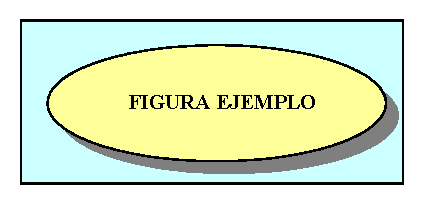
\includegraphics[angle=0,width=0.5\textwidth]{figura1}
    \caption{This is the caption of the sample figure.}
    \label{fig:sample}
  \end{center}
\end{figure}

\begin{table}[hb]
  \begin{center}
    {\caption{A sample table for a sample file.}\label{tab:sample}}
    \begin{tabular}{|l|l|}
      \hline
      Sample algorithm & Sample performance  \\
      \hline
      A & Bad\\
      \hline
      B & Excellent\\
      \hline
      C & Unstable\\
      \hline
      D & Unforgettable\\
      \hline
    \end{tabular}
  \end{center}
\end{table}

\section{References}
References should be clear and complete. Sample references are these
\cite{pearl1984} \cite{hartetal1968} \cite{korf1985} and this one
\cite{oetikeretal2008}. Do not forget to include DOI numbers in your
references when available. You can associate hyperlinks to DOI numbers
in \LaTeX using the \textbackslash doi command, see for example
\cite{vovk2007}. Please, pay attention to the difference with
\cite{oetikeretal2008} that explicitly includes a URL, and not a DOI
reference. See below the format of references. \LaTeX users are
encouraged to use Bibtex.

\subsection{What is a DOI?}
The DOI (Digital Object Identifier) is a unique identifier assigned by
publishers to electronically published items (books, journal papers,
etc.) The DOI system provides a framework for persistent
identification. The physical location of a digital object may change
over time, but its DOI name will not change. Currently, a DOI number
can be resolved prefixing http://dx.doi.org/ to the DOI. Therefore
links of the form http://dx.doi.org/[DOI] are expected to work
properly over time, regardless of the physical location changes of the
referenced items. To learn more about the DOI see
\url{http://www.doi.org}

\subsection{Where can I find the DOI of my references?}
DOI numbers should appear explicitly in the first page of printed
journal papers, either at the top or bottom of the page, like in
figure \ref{fig:print-doi}. Electronic journals display DOI numbers in
the papers access or home pages, like in figure \ref{fig:home-doi}. If
you cannot find the DOI of a reference at first sight it probably does
not have one, so do not worry. Many articles do not have DOI numbers
assigned (specially older ones).

\begin{figure}
  \begin{center}
    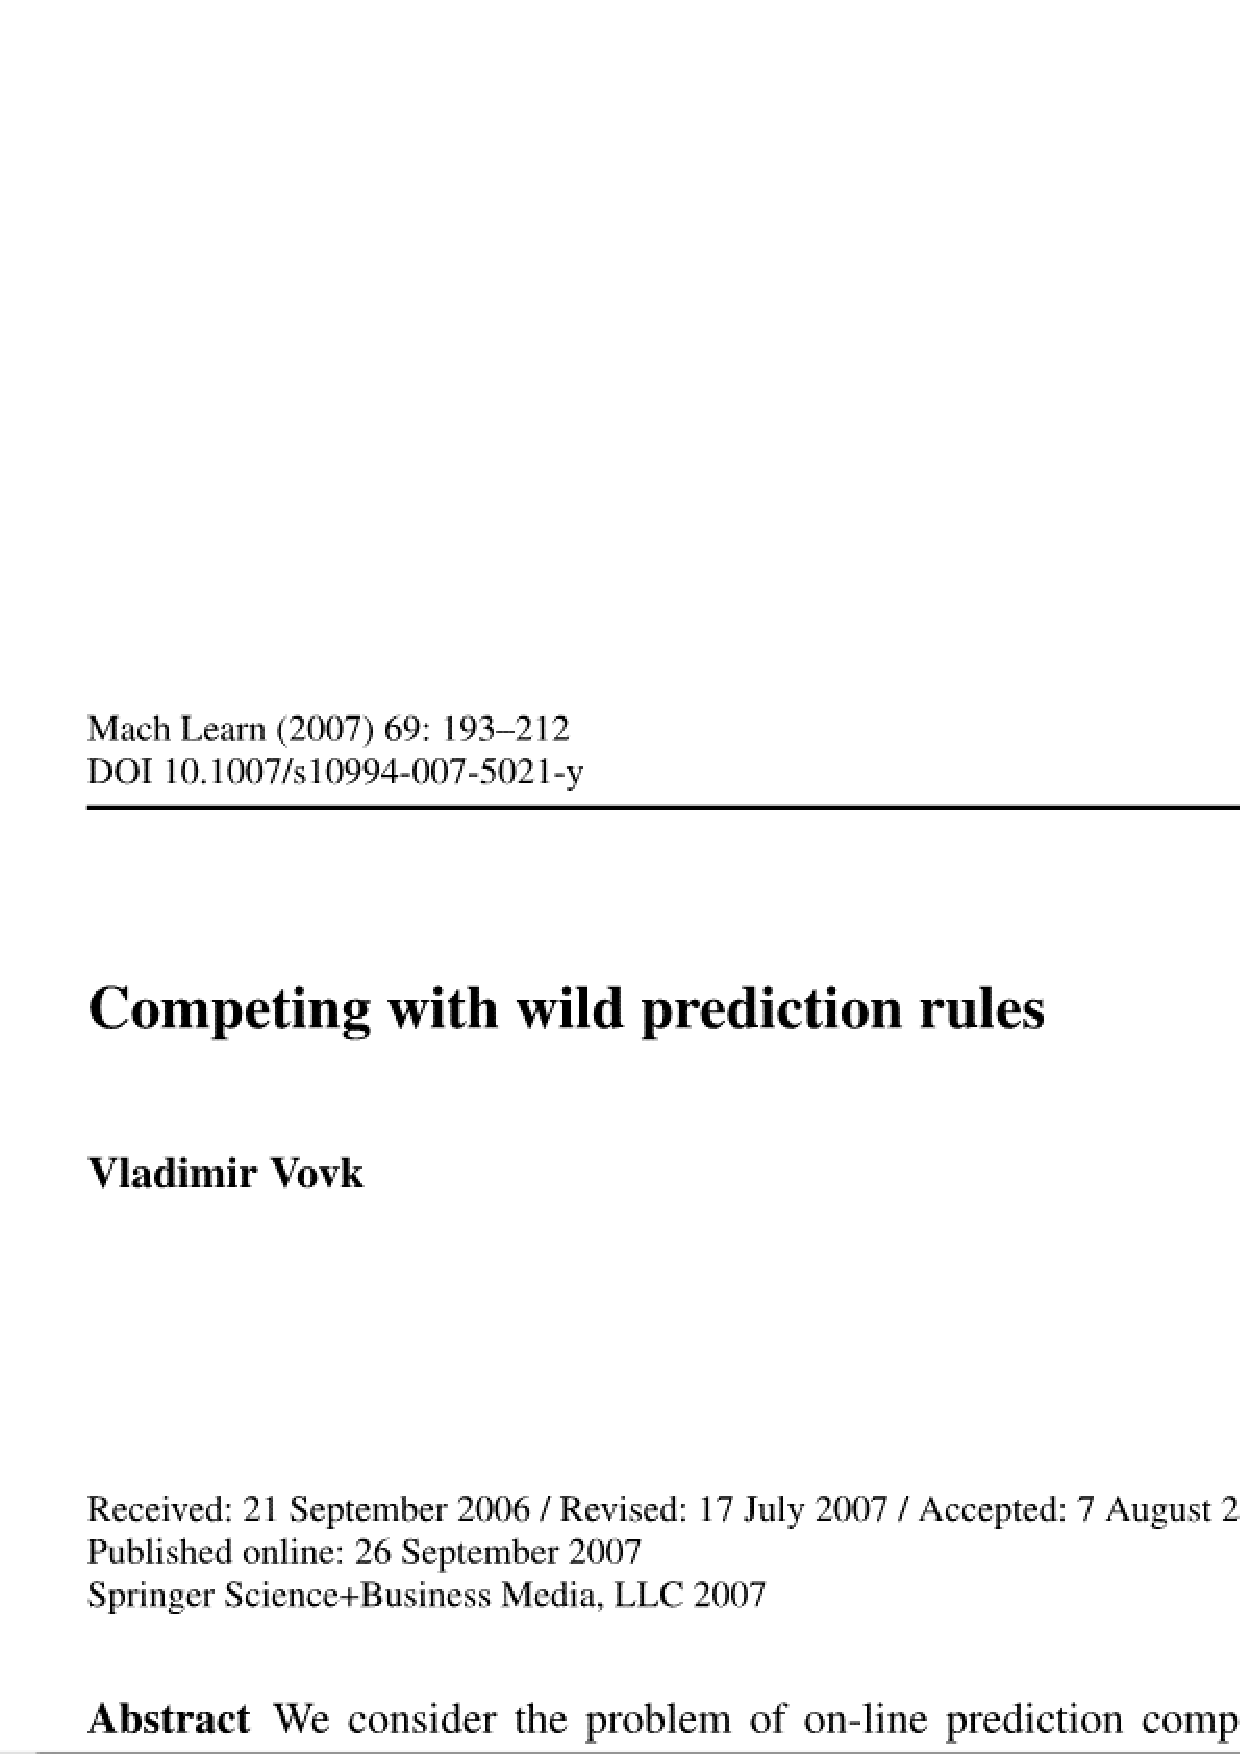
\includegraphics[angle=0,width=0.7\textwidth]{print-doi}
    \caption{DOI in a printed document.}
    \label{fig:print-doi}
 \end{center}
\end{figure}

\begin{figure}
  \begin{center}
    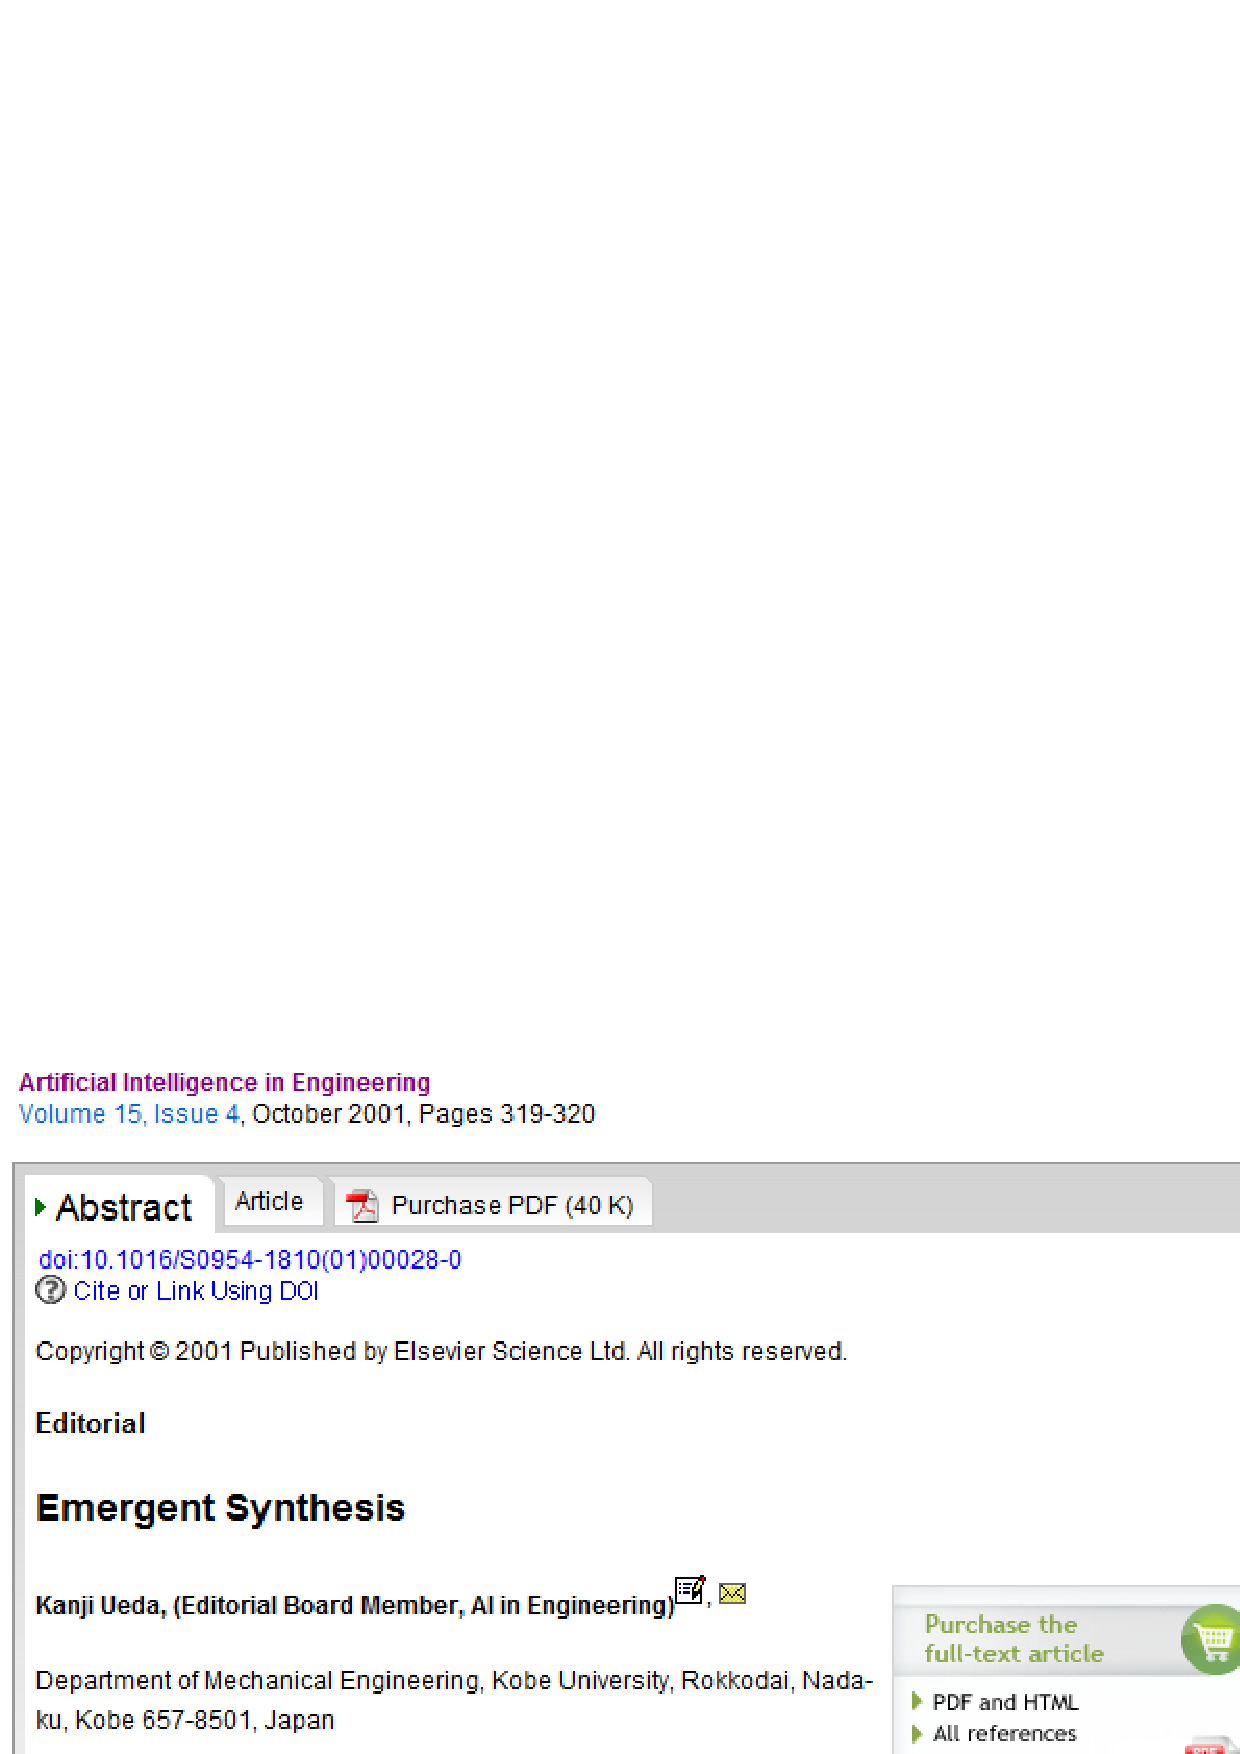
\includegraphics[angle=0,width=0.7\textwidth]{home-doi}
    \caption{DOI in a document available on the Web.}
    \label{fig:home-doi}
 \end{center}
\end{figure}

\subsection{Why is it important to include DOI numbers in references
  (when available)?}

New papers published by Inteligencia Artificial are assigned a DOI
number as a free service to their authors. Documents receiving a DOI
are expected to include DOI numbers in their own references.

Including DOI numbers in your references (when available) will make
your paper more useful and comfortable to read for readers and
reviewers. If you are a \LaTeX user and include DOI numbers as
explained above, the related hyperlinks will be added automatically to
your document.

\section{Journal Scope}
Inteligencia Artificial is a quarterly journal promoted and sponsored by Iberamia (Sociedad Iberoamericana de Inteligencia Artificial)(http://iberamia.dsic.upv.es/inicial.html). The journal publishes high-quality original research papers reporting theoretical or applied advances in all branches of Artificial Intelligence. In addition to rapid publication and dissemination of unsolicited contributions, Inteligencia Artificial is committed to producing monographs and special issues on topics of special relevance to the AI community.

\section{Manuscript Submission and Review}

Paper submission should be carried out through the journal's Web page http://journal.iberamia.org. Click the ``ABOUT'' button and follow the author's guidelines.

Following this process the author implicitly transfers copyright of
accepted papers to IBERAMIA, accepting their publication electronically
(freely available through the Journal's Web pages) and in printed
volumes.

Inteligencia Artificial welcomes research papers written in Spanish or
English. Manuscripts should be uploaded in PDF format through the
journal's Web pages (http://journal.iberamia.org - link 'Submissions').
All research papers falling within the journal's scope will be subject
to double-blind peer-review by at least two anonymous
reviewers. Authors must omit their names in submitted manuscripts. The
journal publishes four issues per year, each one at the start of each
season (spring, summer, autumn, and winter). The journal will not
carry out editing of manuscripts. Authors should adhere strictly to
the norms in the "Journal's formatting guidelines".  Accepted papers
will be published electronically at the journal's Web pages, with free
access from the Internet. The journal encourages authors to add links
in their personal pages pointing to the journal's pages containing
their contributions.

\section{Originality and Copyright}
Research papers submitted to Inteligencia Artificial cannot have been
published previously, nor be under review for publication
elsewhere. However, the journal welcomes extended and improved
versions of papers published in conferences and workshops, which will
be subject to a new peer-review process.  Authors implicitly accept
publication of submitted papers by , both electronically (with
free access from the Internet) and in print, as well as dissemination
through other media and entities with which IBERAMIA may establish
agreement, transferring IBERAMIA all the necessary rights.

\section{Monographs and Special Issues}
The journal welcomes monograph or special issue proposals related to
specific areas of Artificial Intelligence. Proposals to coordinate
monographs or special issues should be sent through email to the
Editor (editor@iberamia.org).  Contributions to monographs or special
issues can be original works including new research papers, extended
and improved versions of papers published in conferences and
workshops, and survey papers that summarize the topics of a particular
monograph or special issue. In all cases, the publication of
contributions is conditioned to acceptance in a new peer-review
process carried out by an international scientific committee under the
journal's supervision.

\section{Theses Summaries }
Inteligencia Artificial is specially interested in the publication of
Ph.D. dissertation summaries that provide a quick and state-of-the-art
reference in particular topics of Artificial Intelligence. Summaries
can be submitted following the regular submission process, stating
"RESUMEN DE TESIS" in the heading, and should be limited to 2-4 pages.


\section*{Acknowledgements}
This is the place for acknowledgements.

\bibliographystyle{plain}
\bibliography{iberamia}         %Check the iberamia.bib file

\end{document}
